\chapter{Evaluations} 
\label{chap:refs}
\label{chap:ch5_abbr}
\section{Test cases}
We have evaluated this software by testing different functionality as specified in the requirement. This was achieved by creating multiple cases that proves the performance of the software. This evalution was performed in real time and directly online. We have inlcuded images and table showing the test cases and results. 
\section*{Checking Available Machines}
In the software specification, it is designed to have search option on the user interface. One of this search requirement is to check for available machines (unreserved machines). In the below table is list of machines reserved for different date. The test is to enter a search query with a specific date interval and ask the software to provide any machine available withing that date.

\begin{table}[h!]
  \centering
  \label{tab:table1}
  \begin{tabular}{l|c||c||c||c||c||c||r}
    No & Machines & Aug & Sep & Oct & Nov & Dec & Jan \\
    \hline
    1 &Machine A & free & free & free & free & free & free\\
    2 &Machine B & free & free & free & 1st to 30th & free & free\\
    3 &Machine C & 17th - & - & - & 24 & free & free\\
    4 &Machine D & 25 & - & 25 & free & free & free\\
    5 &Machine E & free & free & 1st to 31st & free & free & free\\
    6 &Machine F & free & free & free & free & 2nd to 31st & free\\
  \end{tabular}
  \caption{List of Reservations}
\end{table}

\begin{table}[h!]
  \centering
  \label{tab:table1}
  \begin{tabular}{l|c||r}
    No & Date: start --- end & Available machines\\
    \hline
    1 &12-08-2017 to 30-08-2017  & A B E F \\
    2 &17-08-2017 to 24-08-2017  & A B D E F\\
    3 &01-08-2017 to 05-10-2017  & A B F \\
    4 &05-08-2017 to 10-08-2017  & A F \\
    5 &01-08-2017 to 30-08-2017  & A D E  \\
    6 &01-01-2018 to 30-01-2018  & A B C D E F \\
  \end{tabular}
  \caption{test 1}
\end{table}

\begin{table}[h!]
  \centering
  \label{tab:table1}
  \begin{tabular}{l|c||r}
    No & Date: start --- end & Available machines\\
    \hline
    1 &01-08-2017 to 01-01-2018  & A \\
    2 &01-08-2017 to 15-11-2017  & A F\\
    3 &01-12-2017 to 30-01-2018  & B C A D E \\
    4 &30-11-2017 to 30-12-2017  & A  C D E\\
    5 &02-10-2017 to 02-08-2017  & A  D E \\
   
  \end{tabular}
  \caption{test 2}
\end{table}

\section*{Reserving a machine}
Reserving machine is another requirement we have implemented in this software. This is the process where users choose and reserve a machine for definit time and date. When a reservation is made, the details of the reservation appears under the machine being reserved. Figure \ref{fig:reserve} shows the evaluting of this function, where we put details of reservation, by selecting a username, machine and inserting start and end time/date. After submiting with the reserve button, the it appears on the inventory with other reservations list. 
\pagebreak
\begin{figure}[h]
  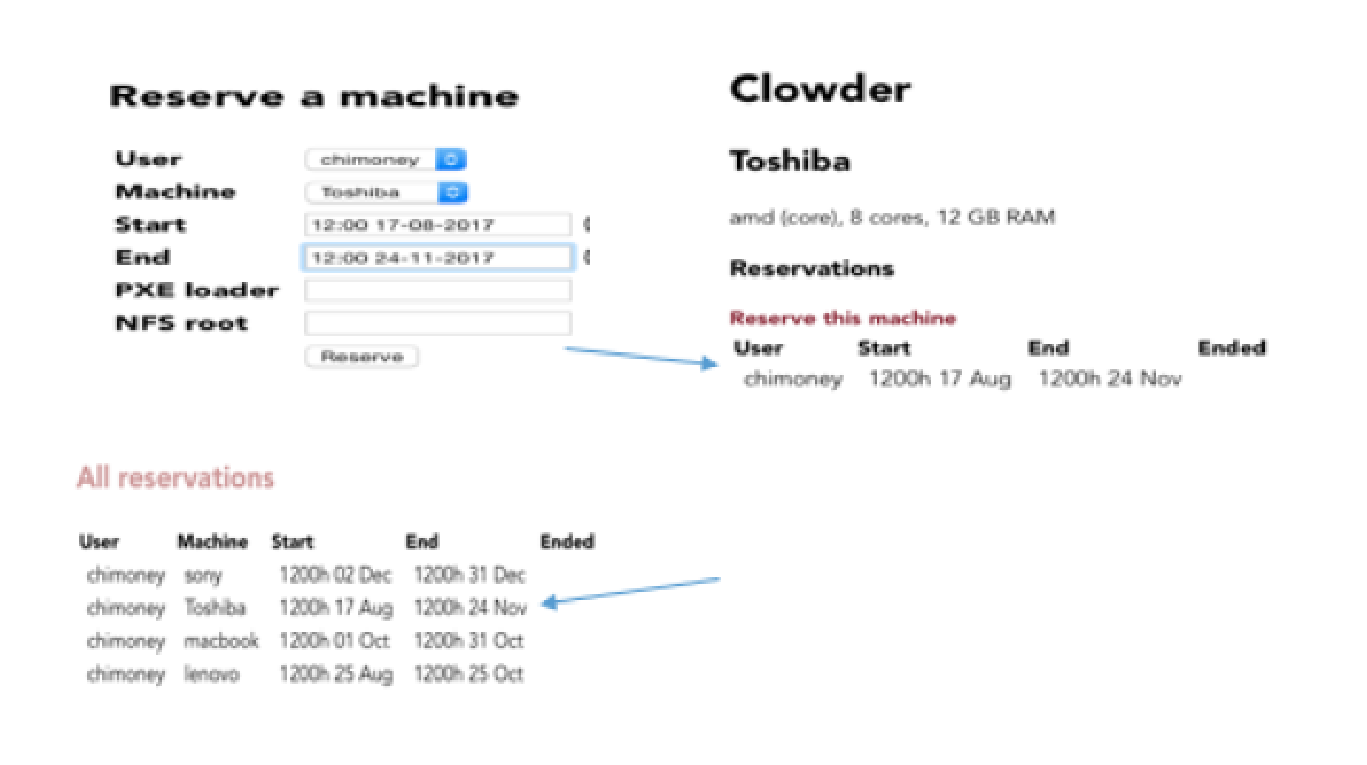
\includegraphics[width=\linewidth]{reserve.eps}
  \label{fig:reserve}
  \caption{Reservation function}
\end{figure}

\section*{Updating a machine}
Update functionality allow users to change the details of a machine already stored in the database. This is to enable them update the information about each machine as needed when ever there is an upgrade in the system. We have tested this functionality by changing the entire information of a machine listed in the inventory. Figure \ref{fig:reserve}  shows an example of this test case.

\begin{figure}[h]
  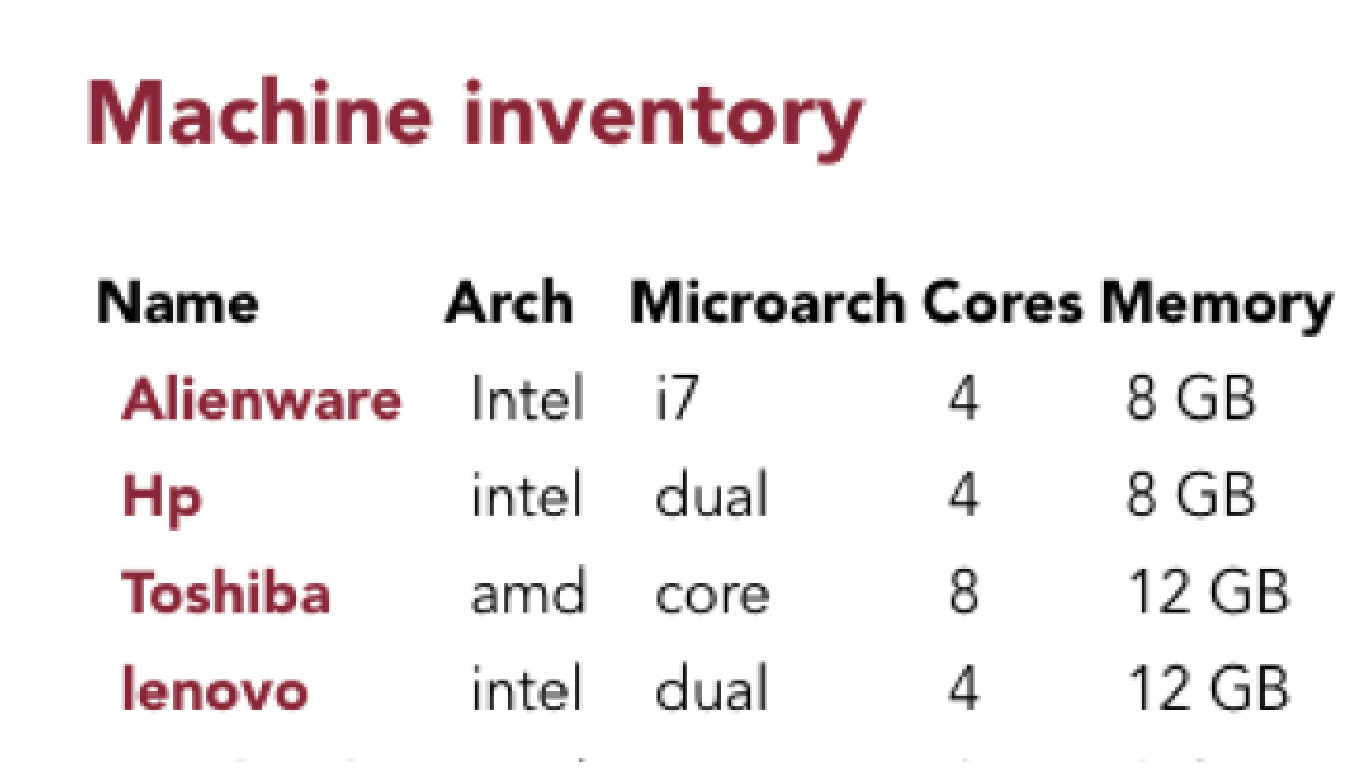
\includegraphics[width=\linewidth]{update.eps}
  \label{fig:reserve}
  \caption{Before update}
\end{figure}


\begin{figure}[h]
  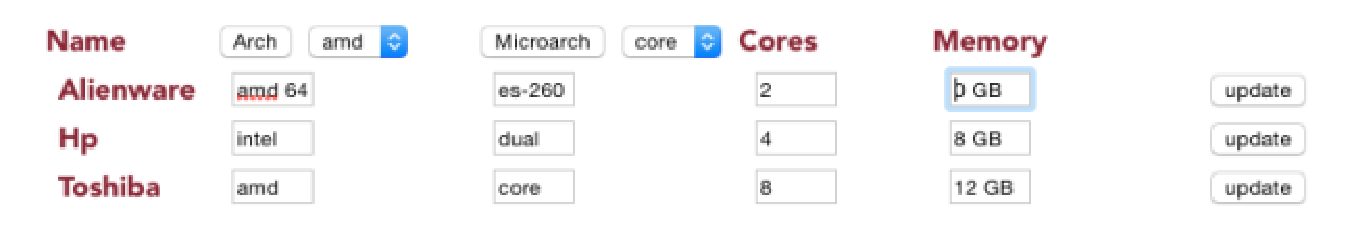
\includegraphics[width=\linewidth]{change.eps}
  \label{fig:reserve}
  \caption{Editing machine details}
\end{figure}

\begin{figure}[h]
  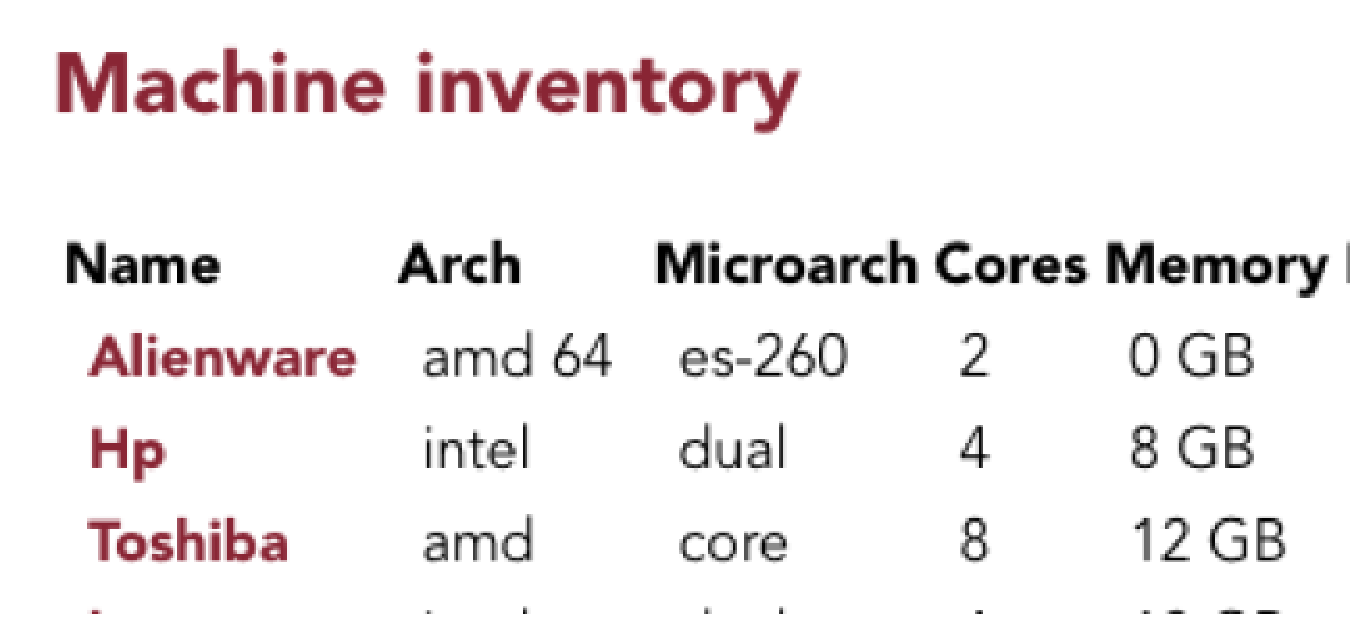
\includegraphics[width=\linewidth]{update2.eps}
  \label{fig:reserve}
  \caption{Updated machine properties}
\end{figure}
\pagebreak

\section*{filtering inventory}
This functionality helps user to filter the inventory using the context of desired information. User is able to filter the machines inventory with memory size. The size range is inserted in the search to get the list of machines that fall within the range. When the button is clicked, the  server returns the list of machine that falls in the range. Another type of filtering is the the drop list filter. This type has a dropdown menu user select a context option to search for. For exaple, user can filter the machine inventory by selecting type os microarchitectre and architect..\begin{figure}[h]
  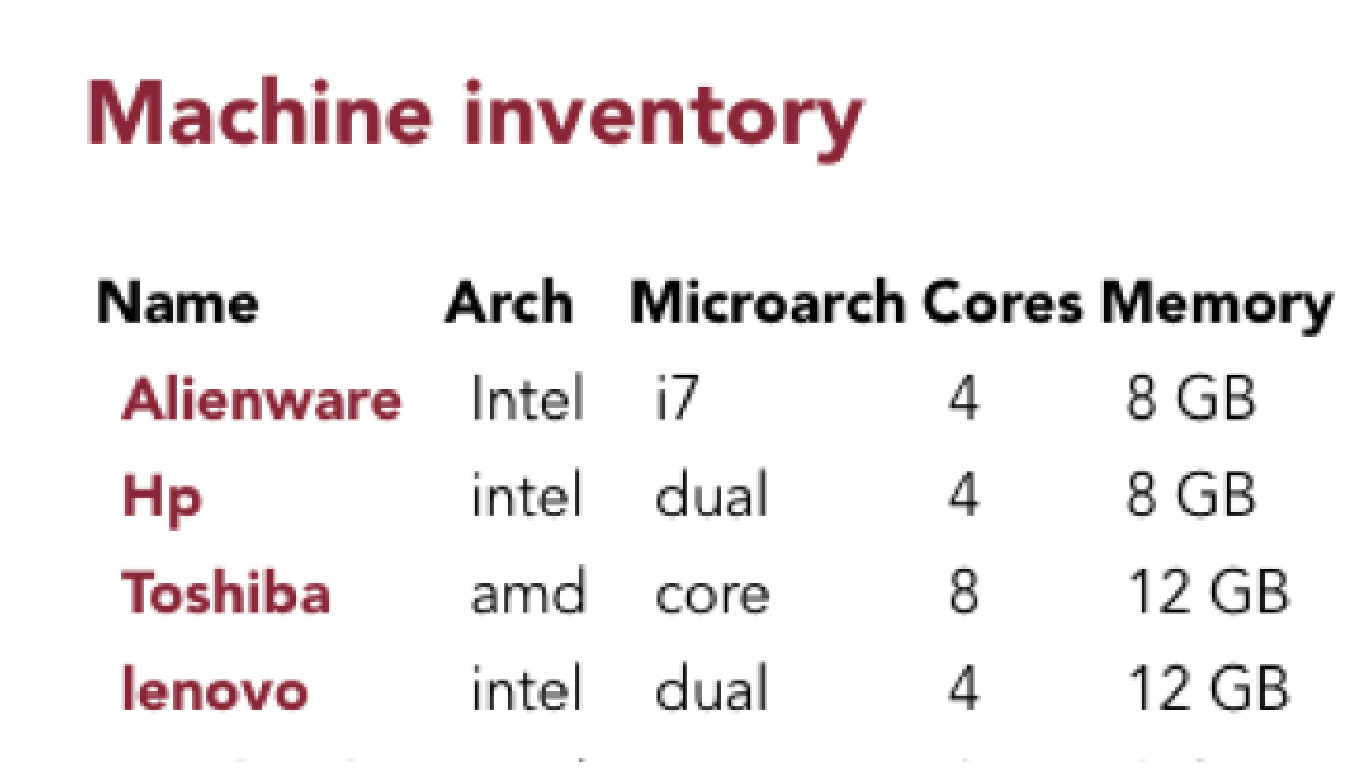
\includegraphics[width=\linewidth]{update.eps}
  \label{fig:reserve}
  \caption{Reservation function}
\end{figure}
\pagebreak


\section{Evaluations}
